% !TeX spellcheck = pl_PL
\newpage
\section{Bluetooth}
\subsection{Właściwości}
\begin{itemize}
	\item Bezprzewodowy system komunikacyjny
	\item Krótki zasięg zestawiony "ad-hoc"
	\item \textit{Pikonet}: sieć personalna (WPAN) oparta o master-slave
	\begin{itemize}
		\item Można wyróżnić slave'y aktywne i zaparkowane
		\item Dwa rodzaje połączeń: z aktywnym i zaparkowanym
		\item Połączenie z zaparkowanym slave'ie nie wymienia informacji, ale utrzymuje informacje o urządzeniu i aktualizuje jego status (np. jak urządzenie wyjdzie poza zasięg pikonetu to nie przestaje być uwzględniane).
	\end{itemize}
	\item Możliwości:
	\begin{itemize}
		\item Współpraca osobistych urządzeń użytkownika
		\item Podłączenie urządzeń do sieci (przez punkty dostępowe np.)
		\item Automatycznie się kompiluje, wykonuje procedury konfiguracyjne przygotowujące system do komunikacji.
		\item Automatyczne:
		\begin{itemize}
			\item Wyszukiwanie urządzeń (\emph{inquiring}) - stwierdzanie, że w zasięgu znalazło się nowe urządzenie i wykonuje odpowiednią konfiguracje by włączyć je do pikonetu. Może to być wykonywane zarówno przez mastera, jak i slave (?).
			\item Podłączenie do mastera (\emph{paging}) - jak pojawia się zgoda na bycie wykrytym, tworzy połączenie fizyczne pozwalające na przesył danych między M-S.
			\item Wykrywanie usług
		\end{itemize}
	\end{itemize}
	\item Bezpieczeństwo komunikacji: uwierzytelnianie urządzeń i szyfrowanie (\emph{pairing})
	\item Może współpracować w środowiskach silnie zakłóconych (dla systemów w bliskim sąsiedztwie i działających na tym samym paśmie (chyba)	
\end{itemize}
\subsection{Konfiguracja}
\begin{enumerate}
	\item Wyszukiwanie urządzeń (\emph{inquiry})
	\begin{itemize}
		\item Master cyklicznie wysyła komunikat \emph{inquiry}. Istnieje możliwość wyszukiwania urządzeń tylko określonego typu.
		\item Urządzenia wykrywalne po rozpoznaniu \emph{inquiry} odsyłają kilkakrotnie unikatowy adres BT, ale dopiero po odczekaniu losowego czasu. Niewykrywalne po prostu ignorują ten komunikat.
		\item Format:
		\begin{itemize}
			\item MASTER $ Inquiry\:B \rightarrow $ urządzenie BT - rozgłoszenie (\emph{broadcast})
			\item MASTER $ Adres \leftarrow R $ urządzenie BT - losowo opóźniona odpowiedź
		\end{itemize}
		\item Jak urządzenie nie zostaje wykryte, to brak odpowiedzi.
	\end{itemize}
	\item Podłączenia urządzeń (\emph{paging})
	\begin{itemize}
		\item \emph{Paging} wykonywany jest sekwencyjnie na wyznaczonych do tego urzadzeniach. Służy m.in. do synchronizacji urządzeń w zakresie \textbf{czsu}, \textbf{fazy}, \textbf{aktualnego przeskoku częstotliwości}.
		\item Urządzenie po wykonaniu pagingu jest w stanie CONNECTION (podłączenie do mastera) i staje się członkiem pikonetu.
		\item Format:
		\begin{itemize}
			\item MASTER $ Page \rightarrow $ urządzenie BT
			\item MASTER $ Connect\:B \leftarrow $ urządzenie BT
		\end{itemize}
		\item Niewykryte urządzenie pozostaje poza zasięgiem.
	\end{itemize}
\end{enumerate}
\subsection{Przeskoki częstotliwości}
\begin{itemize}
	\item Łącze zostaje podzielone na sloty o czasie trwania $ 625 \mu s $
	\item Przesyłanie informacji parami:
	\begin{itemize}
		\item Przesyłanie $ M \rightarrow $ S odbywa się w szczelinach parzystych
		\item Szczeliny nieparzyste zajęte są na przekazanie odpowiedzi
	\end{itemize}
	\item Brak informacji o takcie między urządzeniami - master i slave potrzebuję oboje zegara do wyznaczania czasu szczelin.
	\begin{itemize}
		\item W czasie pagingu pojawia się ta informacja - przekazana jako jeden z parametrów pagingu (slave dostosowuje się do mastera)
		\item każdy pakiet na bieżąco przekazuje informacje o takcie - \textbf{w każdym slocie obowiązuje \underline{inna} częstotliwość}
	\end{itemize}
	\item Master określa sekwencję przeskoków podczas normalnej transmisji
	\item Slave określa sekwencję przeskoków podczas pagingu
	\item Pasmo ISM: $ 2.4 $ do $ 2.483 $ GHz
	\item Ograniczone dostępne moce: 1; 2.5; 100 [mW].
\end{itemize}

\subsection{Parametry}
\subsubsection{Moc nadajników BT}
\begin{itemize}
	\item Klasa 1: 100 mW (20 dBm), zasięg $ \approx 100 $ m
	\item Klasa 2: 2.5 mW (4 dBm), zasięg $ \approx 10 $ m
	\item Klasa 3: 1 mW (0 dBm), zasięg $ \approx 1 $ m
\end{itemize}
\subsubsection{Modulacja}
GFSK (Gaussian Frequency Shift Keying)\\
\begin{itemize}
	\item Stan logiczny 1 - przesunięcie częstotliwości o 115 kHz w górę względem nośnej
	\item Stan logiczny 0 - przesunięcie częstotliwości o 115 kHz w dół względem nośnej
\end{itemize}
\subsubsection{Szybkość bitowa}
\begin{itemize}
	\item 1 Mb/s dla GFSK (możliwa do osiągnięcia szybkość „średnia”: 723,4 kb/s)
	\item 2 Mb/s dla pi/4-QPSK
	\item 3 Mb/s dla 8-DPSK
\end{itemize}


\subsection{Adres urządzenia}
\subsubsection{Format}
\begin{tabular}{|c|c|c|}
	\hline Lower Address Part & Non-significant Address Part & Upper Address Part \\ 
	\hline 24 bity & 16 bity & 8 bitów \\ 
	\hline 
\end{tabular}\\
Łączenie 48 bitów.
\subsubsection{Właściwości}
\begin{itemize}
	\item Adres BT jest unikalny globalnie
	\item Oprócz adresu BT wyróżnia się:
	\begin{itemize}
		\item AM\_ADDR - adres aktywny w pikonecie
		\item 2 adresy urządzenia zaparkowanego:
		\begin{itemize}
			\item PM\_ADDR
			\item AR\_ADDR
		\end{itemize}
	\end{itemize}
\end{itemize}

\subsection{Transmisja}
\subsubsection{Transmisja synchroniczna}
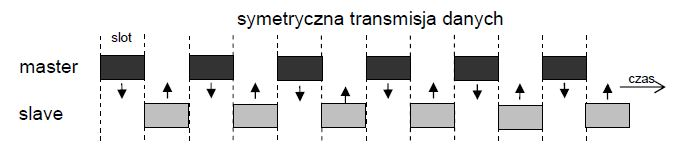
\includegraphics[width=9cm]{./wyklady/bluetooth_2.jpg}\\\\
Dla każdego pakietu jest przewidziany dokładnie taki sam przedział czasu
\subsubsection{Transmisja asynchroniczna}
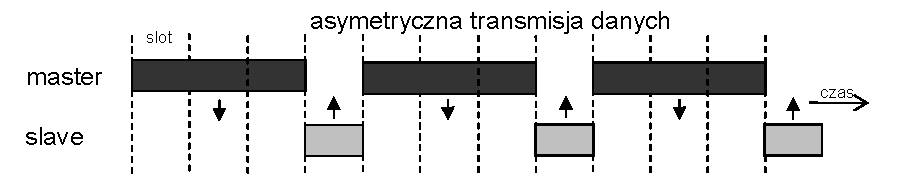
\includegraphics[width=9cm]{./wyklady/Rysunek03.pdf}\\\\
Przedział czasowy obejmuje więcej niż 1 pakiet, maksymalnie do 5 pakietów.

\subsection{Rodzaje danych i łącz}
\subsubsection{Rodzaje danych transmitowanych w BT}
\begin{itemize}
	\item Asynchroniczne
	\item Synchroniczne
	\item Izochroniczne
\end{itemize}
\subsubsection{Rodzaje łącz}
\begin{itemize}
	\item Łącze ACL (bezpołączeniowe - \emph{Connectionless})
	\begin{itemize}
		\item przekazywanie rozkazów zarządzania łączem fizycznym (ACL-C)
		\item przekazywanie asynchronicznych danych użytkownika (ACL-U)
	\end{itemize}
	\item Łącze SCO (połączeniowe -\emph{Connection Oriented})
	\begin{itemize}
		\item Cykliczne przekazywanie danych w zarezerwowanych szczelinach czasowych (stały odstęp miedzy kolejnymi pakietami danego transferu)
		\item Liczba kolejnych szczelin czasowych przydzielonych na transmisję jednego pakietu może wynosić 1, 3 lub 5 (zależy od rodzaju pakietu wybranego dla danego łącza).
	\end{itemize}
	\item Łącze eSCO (połączeniowe -\emph{Connection Oriented})
	\begin{itemize}
			\item podobne do SCO
			\item możliwość retransmisji uszkodzonego pakietu (w tzw. oknie retransmisji)
	\end{itemize}
\end{itemize}

\subsection{Przeskoki częstotliwości}
\emph{Frequency Hopping}
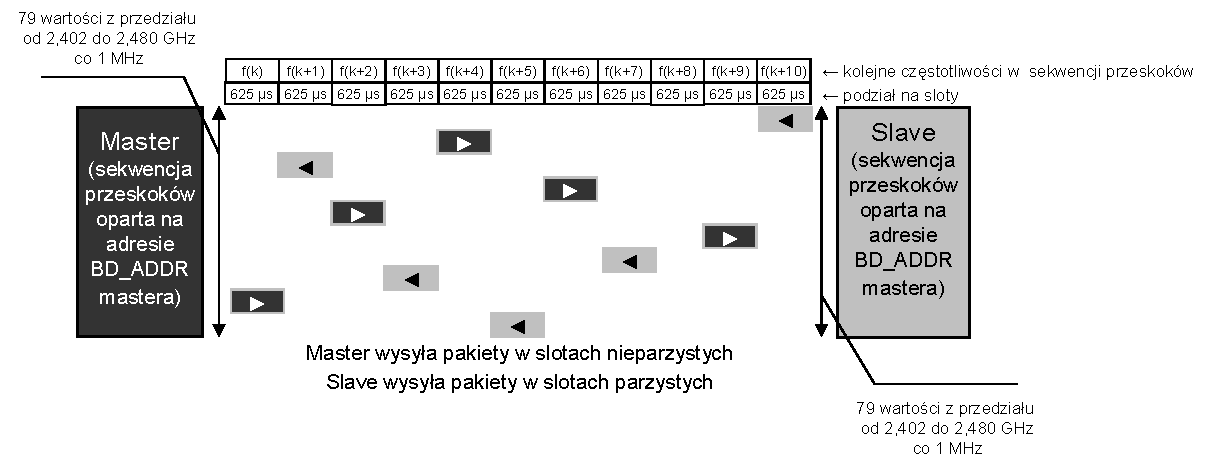
\includegraphics[width=9cm]{./wyklady/Rysunek04.pdf}
\subsubsection{Właściwości}
\begin{itemize}
	\item Występują pomiędzy szczelinami czasowymi
	\item Sekwencja przeskoków musi być znana wszystkim urządzeniom w zasięgu pikonetu
	\item sekwencja przeskoków oparta na adresie BD\_ADDR mastera
	\item 79 wartości z przedziału od 2.402 do 2.480 GHz co 1 MHz
	\item Zastosowanie pesudo-losowych sekwencji przeskoków - zmniejsza to ryzyko zakłóceń.
	\item Im krótsze tym szybsza jest retransmisja informacji.
\end{itemize}
\subsubsection{Adaptacyjne przeskoki częstotliwości}
\begin{itemize}
	\item Polega na wykluczaniu częstotliwości (zakresów pasm) urządzeń uszkodzonych, takich, które bardzo często przekłamują pakiety. Np. zakłócanych przez inną pobliską sieć \textit{pikonet}, albo źródło sygnału wi-fi.
\end{itemize}

\subsection{Pakiety}
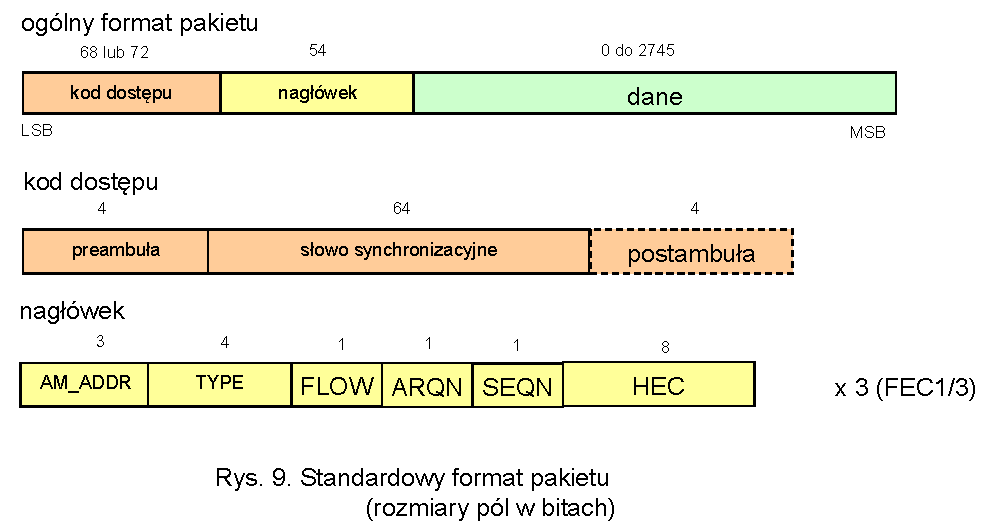
\includegraphics[width=9cm]{./wyklady/Rysunek05.pdf}
\subsubsection{Nagłówek}
Zabezpieczony przez x3 FEC1/3, czyli bity są trzykrotnie duplikowane. \textit{(tryplikowane? XD)}\\
\subsubsection{Kod dostępu}
Preambuła: 0101 lub 1010\\
Słowo synchronizacyjne:
\begin{itemize}
	\item generowane jest na podstawie 24-bitowego LAP
	\item długość: 64 bity
\end{itemize}
Postambuła: 0101 lub 1010\\
Pakiety ID nie mają pola postambuły

\subsection{Zegar}
\begin{itemize}
	\item CLKN - natywny (własny) urządzenia (\emph{native clock})
	\item CLKE - przybliżony (\emph{estimated clock})
	\item CLK - systemowy oparty na zegarze natywnym mastera (\emph{master clock})
\end{itemize}

\subsection{Inquiry i Paging}
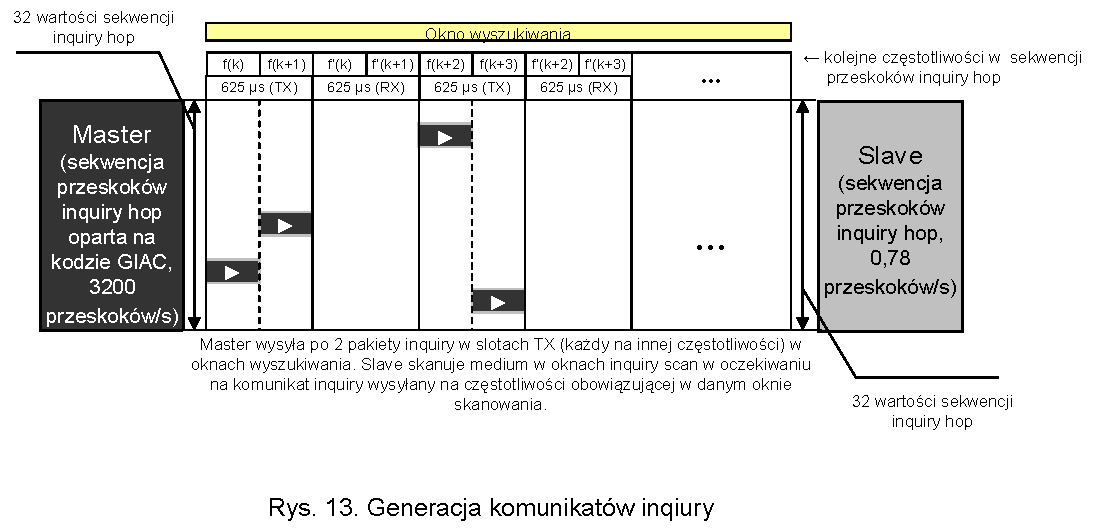
\includegraphics[width=8cm]{./wyklady/Rysunek06.pdf}
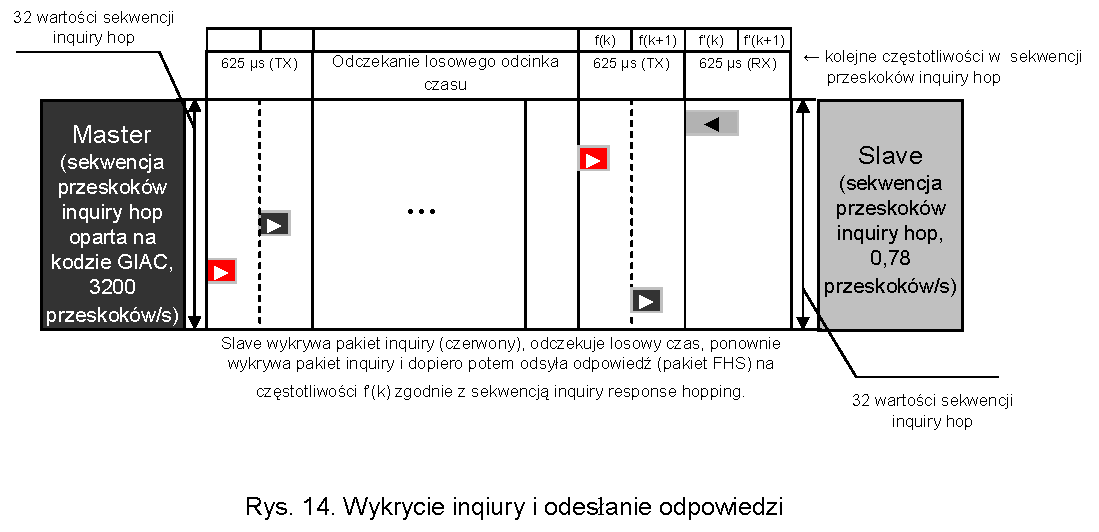
\includegraphics[width=8cm]{./wyklady/Rysunek07.pdf}\\
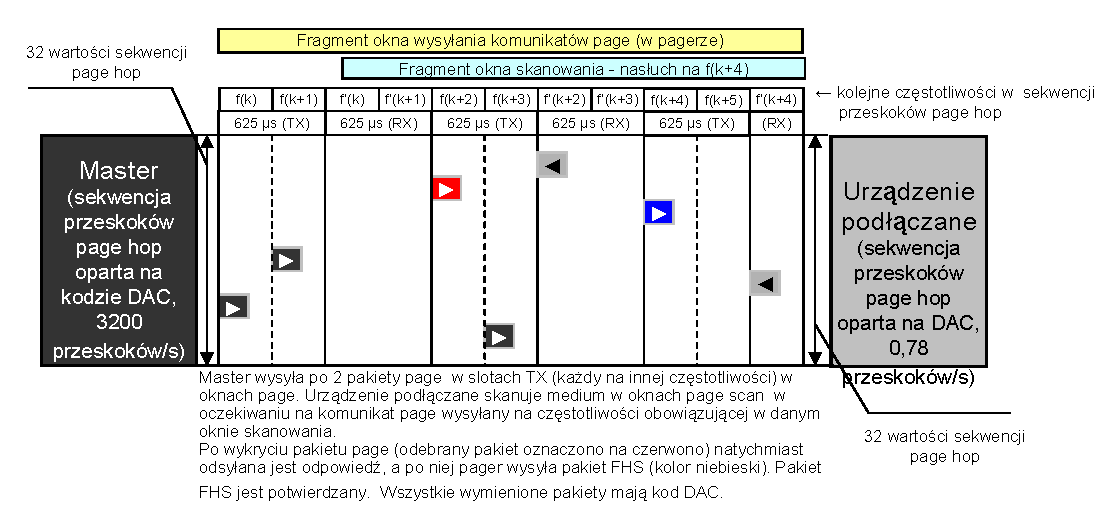
\includegraphics[width=8cm]{./wyklady/Rysunek08.pdf}
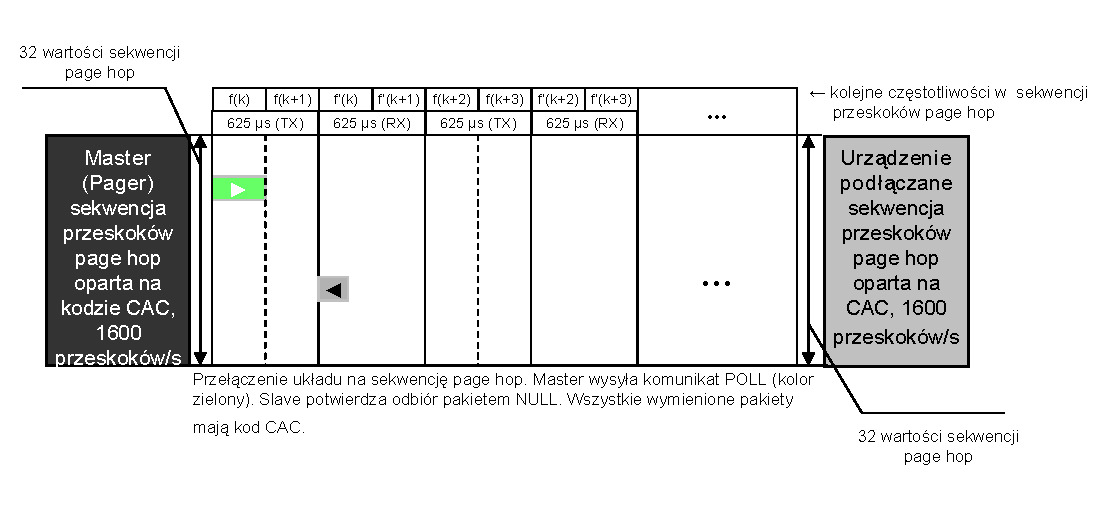
\includegraphics[width=8cm]{./wyklady/Rysunek09.pdf}\\
Generuje komunikaty \emph{inquiry}.
Jak urządzanie odbierze komunikat, to ma obowiązek zwrócenia odpowiedzi. W stałych odstępach czasu wysyła odpowiedź kilkukrotnie - wynika to z tego, że Master może być zajety innymi zadaniami, okno wyszukiwań otwiera tylko raz na jakiś czas.\\
Slave może cały swój wysiłek poświęcić na to, by Master-senpai go zauważył. \\

Rezultatem jest wykrycie urządzenia i pobranie pewnych parametrów, jeżeli master jest chce.\\

Paging: każdy kolejny pakiet jest szyfrowany innym kluczem.

\subsection{Usypianie urządzeń}

\begin{itemize}
	\item \textbf{Tryb HOLD} - blokada łącza ACL na określony czas (zazwyczaj połączony z uśpieniem urządzenia).
	Blokada ma charakter jednorazowy, ale może być powtarzana.
	\item \textbf{Tryb SNIFF} - cykliczna blokada łącza ACL (zazwyczaj połączona z uśpieniem urządzenia)..
	Kolejne blokady łącza są rozdzielone krótkimi interwałami nasłuchu, w których slave oczekuje na zaadresowane do niego pakiety.
	\item \textbf{Stan PARK} - ogranicza do minimum komunikację stacji slave ze stacją master.
	Łącze ACL do stacji slave zostaje trwale zablokowane, slave traci swój adres AM\_ADDR i przechodzi
	do „zaparkowania”.
\end{itemize}

W trybach HOLD i SNIFF slave zachowuje AM\_ADDR i nie przestaje być członkiem pikonetu.Nadal aktywne pozostają łącza SCO i eSCO. \\
W stanie PARK urządzenie otrzymuje dwa adresy zaparkowania, umożliwiające powrót do pikonetu.Podczas parkowania utrzymywana jest synchronizacja mastera z urządzeniem, utrzymywana za pomocą
specjalnego kanału rozgłoszeniowego o nazwie \textit{beacon}.

\subsection{Bezpieczeństwo}

Za bezpieczny system komunikacyjny można uważać taki, który umożliwia poufną wymianę danych pomiędzy urządzeniami o potwierdzonej tożsamości.
Mechanizmy związane z bezpieczeństwem w sieci Bluetooth: 
\begin{itemize}
	\item Parowanie urządzeń (pairing)
	\item Wiązanie urządzeń (bonding)
	\item Stosowanie kluczy
	\begin{itemize}
		\item klucz urządzenia (unit key)
		\item inicjalizacyjny (initialization key)
		\item połączeniowy (link key)
		\item szyfrujący (encription key)
	\end{itemize}
\end{itemize}